\section{Chemische Reaktion - Physikalischer Vorgang}
\begin{longtable}{|c|c|}
\hline \textsc{Chemische Reaktion} & \textsc{Physikalischer Vorgang} \\
\hline Erhitzen von Zucker & Erhitzen von NaCl \\
Verbrennen von Mg &  \\
Mg + H$_{2}$SO$_{4}$ &  \\
\hline Neue Stoffe mit neuen Eigenschaften & Änderung von Form, Aggregatzustand und Lage \\
\hline
\end{longtable}

Siehe Kapitel \ref{Experimente - Chemische Reaktion - Physikalischer Vorgang} auf
Seite \pageref{Experimente - Chemische Reaktion - Physikalischer Vorgang} (Experimente).
\section{Gesetzmäßigkeiten zum Atombau der chemischen Elemente aus dem PSE}
\begin{longtable}{|c|c|}
\hline \textsc{Name} & \textsc{Bedeutung} \\
\hline Ordnungszahl & Protonenzahl ($p^+$) = Elektron ($e^-$) \\
\hline Hauptgruppennummer\;(senkrecht\; Spalten) & Anzahl der Außene$^-$ (Außenelektronen) \\
\hline Periode (waggerchte Spalten) & Anzahl der \enquote{Schalen} \\
\hline
\end{longtable}

\begin{longtable}{|ccc|}
\hline \textsc{Stoffe vor der Reaktion} && \textsc{Stoffe nach der Reaktion} \\
\hline Ausgangsstoffe (Edukte) & $\stackrel{reagieren\;zu}{\rarrowfill{2.5cm}}$ & Reaktionsprodukten \\
\hline
\end{longtable}

\subsection{\acf{H}}
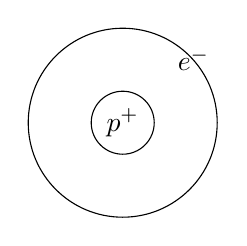
\begin{tikzpicture}[color = {black}]
    \draw[black] (0,0) circle (0.4cm);
    \node (mitte) at (0,0) {$p^+$};
    \draw[black] (0,0) circle (1.2cm);
    \node (c) at (0.9,0.8) {$e^-$};
\end{tikzpicture}
% Immer kleiner Abstände
Sehr reaktionsfreudig
\subsection{\acf{O}}
Abstand der \enquote{Schalen} wird nach außen immer kleiner.\\
\begin{minipage}{5cm}
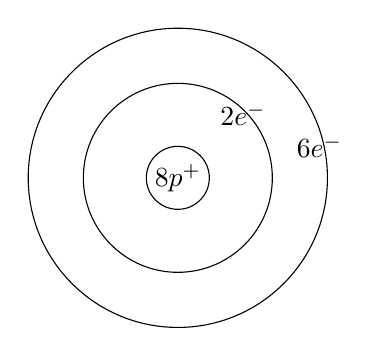
\begin{tikzpicture}[color = {black}]
    \draw[black] (0,0) circle (0.4cm);
    \node (mitte) at (0,0) {$8p^+$};
    \draw[black] (0,0) circle (1.2cm);
    \node (c) at (0.83,0.8) {$2e^-$};
    \draw[black] (0,0) circle (1.9cm);
    \node (c) at (1.8,0.4) {$6e^-$};
\end{tikzpicture}
\end{minipage}
\hfill
\begin{minipage}{10cm}
\vspace{0.25cm}
\begin{list}{}{}
\item[Maximale Schalenbesetzung:] $2n^2 \quad n$ = Schalennummer (es wird von innen nach außen gezählt)
\end{list}
\begin{tabular}{rc}
\textsc{Schalennummer} & \textsc{Außenelektronen} \\
1. & $2e^-$ \\
2. & $8e^-$ \\
3. & $16e^-$ \\
4. & $32e^-$ \\
\end{tabular}
\end{minipage}

\subsection{\acf{Na}}
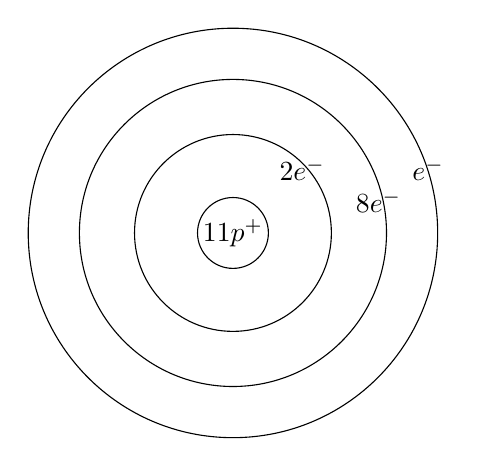
\begin{tikzpicture}[color = {black}]
    \draw[black] (0,0) circle (0.45cm);
    \node (mitte) at (0,0) {$11p^+$};
    \draw[black] (0,0) circle (1.25cm);
    \node (c) at (0.88,0.8) {$2e^-$};
    \draw[black] (0,0) circle (1.95cm);
    \node (c) at (1.85,0.4) {$8e^-$};
    \draw[black] (0,0) circle (2.6cm);
    \node (c) at (2.48,0.8) {$e^-$};
\end{tikzpicture}

\subsection{\acf{Al}}
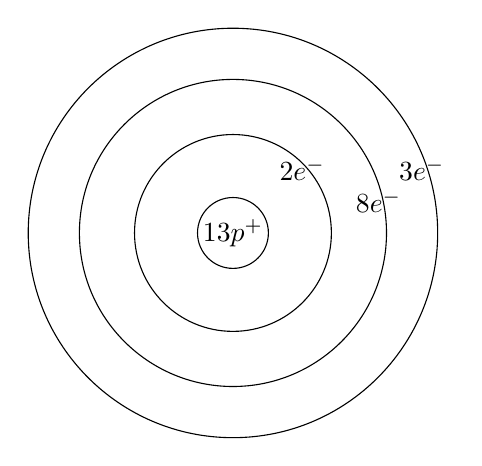
\begin{tikzpicture}[color = {black}]
    \draw[black] (0,0) circle (0.45cm);
    \node (mitte) at (0,0) {$13p^+$};
    \draw[black] (0,0) circle (1.25cm);
    \node (c) at (0.88,0.8) {$2e^-$};
    \draw[black] (0,0) circle (1.95cm);
    \node (c) at (1.85,0.4) {$8e^-$};
    \draw[black] (0,0) circle (2.6cm);
    \node (c) at (2.4,0.8) {$3e^-$};
\end{tikzpicture}
%Atomkern: 0.45     +0.8
%Hülle 1: 1.25      +0.7
%Hülle 2: 1.95      +0.6
%Hülle 3: 2.6       +0.5

\subsection{\acf{Ca}}
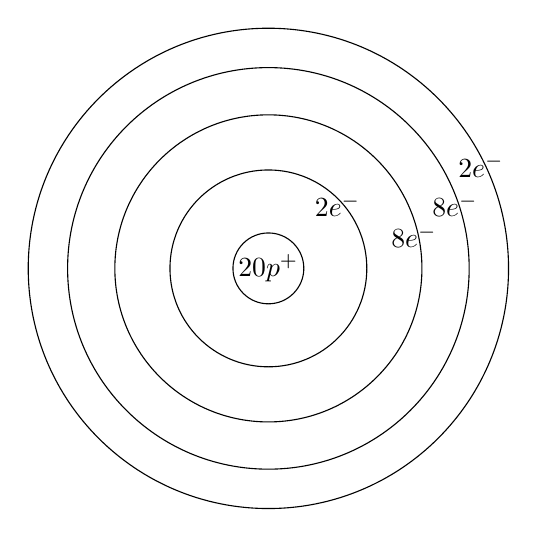
\begin{tikzpicture}[color = {black}]
    \draw[black] (0,0) circle (0.45cm);
    \node (mitte) at (0,0) {$20p^+$};
    \draw[black] (0,0) circle (1.25cm);
    \node (c) at (0.88,0.8) {$2e^-$};
    \draw[black] (0,0) circle (1.95cm);
    \node (c) at (1.85,0.4) {$8e^-$};
    \draw[black] (0,0) circle (2.55cm);
    \node (c) at (2.37,0.8) {$8e^-$};
    \draw[black] (0,0) circle (3.05cm);
    \node (c) at (2.7,1.3) {$2e^-$};
\end{tikzpicture}

\section{Energieniveauschema}
Bei dieser Schreibweise wird der Kern nicht mehr dargestellt und die Anzahl der Protonen, respektive die Ordnungszahl, muss
erst durch das Addieren der Elektronen ermittelt werden.
\subsection{\acf{O}}
\begin{picture}(5,30)
\put(10,32){\makebox(0,0){Energie}}
\put(23,18){\makebox(0,0){$6e^-$}}
\put(49,20){\makebox(0,0){2. Schale}}
\put(23,8){\makebox(0,0){$2e^-$}}
\put(49,10){\makebox(0,0){1. Schale}}
\put(10,10){\line(0,1){20}}
\put(10,10){\line(1,0){30}}
\put(10,20){\line(1,0){30}}
\end{picture}
\subsection{\acf{Na}}
\begin{picture}(5,40)
\put(10,42){\makebox(0,0){Energie}}
\put(23,28){\makebox(0,0){$1e^-$}}
\put(49,30){\makebox(0,0){3. Schale}}
\put(23,18){\makebox(0,0){$8e^-$}}
\put(49,20){\makebox(0,0){2. Schale}}
\put(23,8){\makebox(0,0){$2e^-$}}
\put(49,10){\makebox(0,0){1. Schale}}
\put(10,10){\line(0,1){30}}
\put(10,10){\line(1,0){30}}
\put(10,20){\line(1,0){30}}
\put(10,30){\line(1,0){30}}
\end{picture}
\subsection{\acf{Ca}}
\begin{picture}(5,50)
\put(10,52){\makebox(0,0){Energie}}
\put(23,38){\makebox(0,0){$2e^-$}}
\put(49,40){\makebox(0,0){4. Schale}}
\put(23,28){\makebox(0,0){$8e^-$}}
\put(49,30){\makebox(0,0){3. Schale}}
\put(23,18){\makebox(0,0){$8e^-$}}
\put(49,20){\makebox(0,0){2. Schale}}
\put(23,8){\makebox(0,0){$2e^-$}}
\put(49,10){\makebox(0,0){1. Schale}}
\put(10,10){\line(0,1){40}}
\put(10,10){\line(1,0){30}}
\put(10,20){\line(1,0){30}}
\put(10,30){\line(1,0){30}}
\put(10,40){\line(1,0){30}}
\end{picture}
\section{Lewis-Schreibweise}
Auch als Außenelektronschreibweise oder Schreibweise mit allen bindenden und nicht bindenden $e^-$ bekannt.

Da in der Regel nur die Außenelektronen reagieren, führte man diese Schreibweise ein.

\begin{picture}(50,30)
%\put(16,15){\line(1,-5){2}}
%\put(16,7){\line(2,-5){2}}
\put(15.7,23){\line(-1,-5){1.8}}
\put(15.7,23){\line(-3,-5){3.8}}
\put(6.5,1.5){\line(1,5){1.8}}
\put(6.5,1.5){\line(2,5){3}}
\put(11,15.5){\circle*{0.8}}
\put(13.5,12.9){\circle*{0.8}}
\put(15,25){\makebox(5,2){bindende $e^-$}}
\linethickness{0.3mm}
\put(8.5,12){\line(0,0){2}}
\put(10,10.5){\line(1,0){2}}
\put(11,13){\makebox(0,0){O}}
\put(21,-1){\makebox(5,2){nicht bindende $e^-$-Paare}}
\end{picture}

\begin{picture}(20,25)
\put(15,12.9){\circle*{0.8}}
\put(11.5,13){\makebox(0,0){Na}}
\end{picture}Sehr reaktionsfreudig

\begin{picture}(50,25)
\put(15,12.9){\circle*{0.8}}
\put(8,12.9){\circle*{0.8}}
\put(11.5,13){\makebox(0,0){Ca}}
\end{picture}
\section{Verbinden von Stoffen}
\begin{picture}(50,15)
\linethickness{0.3mm}
\put(12.45,12.9){\line(1,0){2}}
\put(11,13){\makebox(0,0){H}}
\put(16,13){\makebox(0,0){H}}
\put(13.6,6){\makebox(0,0){Molekül}}
\put(45,10){\makebox(0,0){He}}
\end{picture}
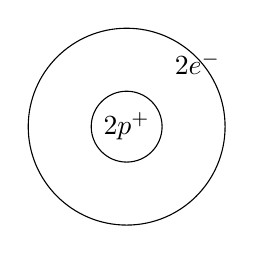
\begin{tikzpicture}[color = {black}]
    \draw[black] (0,0) circle (0.45cm);
    \node (mitte) at (0,0) {$2p^+$};
    \draw[black] (0,0) circle (1.25cm);
    \node (c) at (0.9,0.8) {$2e^-$};
\end{tikzpicture}

Moleküle sind die kleinsten Teilchen chemischer Verbindungen, sie bestehen mindestens aus zwei Atomen.

Alle Elemente folgen der Oktettregel: Alle Atome haben das Bestreben, eine voll besetzte Außenschale zu besitzen um einen
stabilen, energiearmen Zustand zu erreichen.\\
Ausnahme: Heliumzustand

\begin{picture}(50,30)
\linethickness{0.3mm}
\put(9.5,15.5){\line(1,0){2}}
\put(13.5,12.9){\line(1,0){2}}
\put(8.1,12){\line(0,0){2}}
\put(9.5,10.5){\line(1,0){2}}
\put(11,13){\makebox(0,0){Cl}}
\put(18,13){\makebox(0,0){Cl}}
\put(17,15.5){\line(1,0){2}}
\put(20.7,12){\line(0,0){2}}
\put(17,10.5){\line(1,0){2}}
%
\put(48.5,12){\line(0,0){2}}
\put(53.5,13.9){\line(1,0){2}}
\put(53.5,12.9){\line(1,0){2}}
\put(53.5,11.9){\line(1,0){2}}
\put(51,13){\makebox(0,0){N}}
\put(58,13){\makebox(0,0){N}}
\put(60.7,12){\line(0,0){2}}
\end{picture}

\subsection{Reine Atombindung}
Reine Atombindung ist eine chemische Verbindung zwischen zwei gleichen Atomen. Die Protonen des Atomkerns ziehen die
Elektronen des Partners an. Er ist die schwächste bekannte Bindungsart. Die Stoffe sind gasförmig oder flüssig, dann leicht
flüchtig.

\subsection{Polare Atombindung}
Chemische Verbindung zwischen verschiedenartigen Nichtmetallatomen, wobei ein Partner das bindende $e^-$-Paar stärker zu
sich zieht. Es entstehen Teilladungen.

\begin{picture}(50,30)
\linethickness{0.3mm}
\put(12,13){\makebox(0,0){H}}
\put(14.5,13){\makebox(0,0){$\lhd$}}
\put(18,13){\makebox(0,0){Cl}}
\put(17,15.5){\line(1,0){2}}
\put(20.7,12){\line(0,0){2}}
\put(17,10.5){\line(1,0){2}}
%
\linethickness{0.3mm}
\put(52,13){\makebox(0,0){H}}
\put(50,16){\makebox(0,0){$\delta^+$}}
\put(53.6,13){\line(1,0){2}}
\put(58,13){\makebox(0,0){Cl}}
\put(63,16){\makebox(0,0){$\delta^-$}}
\put(57,15.5){\line(1,0){2}}
\put(60.7,12){\line(0,0){2}}
\put(57,10.5){\line(1,0){2}}
\end{picture}

\section{Chemische Zeichenprache}
\begin{itemize}
\item Symbole:
\begin{itemize}
\item Abkürzung für Elemente
\item Ein Atom des Elementes
\end{itemize}

\item Element: Stoff, der nur aus einer Atomart besteht

\item Formeln:
\begin{itemize}
\item Abkürzungen für chemische Verbindungen
\item Angabe des Zahlenverhältnisses für die kleinste Einheit einer chemischen Verbindung.

\end{itemize}
\item Wertigkeit: Zahl die angibt, wie viel Wasserstoff-Atome eines Elements binden oder in einer Verbindung ersetzten
kann.
Es gibt auch Stoffe, die verschiedene Wertigkeiten haben.

H ist immer einwertig: $\stackrel{\RM{1}}{H}$

O ist immer zweiwertig: $\stackrel{\RM{2}}{O}$

\begin{picture}(20,20)
\linethickness{0.3mm}
\multiput(30,10)(0,4){2}{\line(1,0){8}}
\multiput(30,10)(8,0){2}{\line(0,0){4}}
\multiput(33,11)(2,0){2}{\line(0,0){2}}
\put(26,12){\makebox(0,0){O:}}
%
\multiput(30,3)(0,4){2}{\line(1,0){3}}
\multiput(30,3)(3,0){2}{\line(0,0){4}}
\multiput(35,3)(0,4){2}{\line(1,0){3}}
\multiput(35,3)(3,0){2}{\line(0,0){4}}
\put(31.5,4){\line(0,0){2}}
\put(36.5,4){\line(0,0){2}}
\put(26,5){\makebox(0,0){H:}}
%
\put(50,8){\makebox(0,0){$H_2O$}}
\end{picture}

\begin{picture}(50,15)
\linethickness{0.3mm}
\multiput(30,10)(0,4){2}{\line(1,0){14}}
\multiput(30,10)(14,0){2}{\line(0,0){4}}
\multiput(33,11)(2,0){5}{\line(0,0){2}}
%
\multiput(46,10)(0,4){2}{\line(1,0){14}}
\multiput(46,10)(14,0){2}{\line(0,0){4}}
\multiput(49,11)(2,0){5}{\line(0,0){2}}
\put(26,12){\makebox(0,0){P:}}
%%
\multiput(30,3)(0,4){2}{\line(1,0){5}}
\multiput(30,3)(5,0){2}{\line(0,0){4}}
\multiput(31.5,4)(2,0){2}{\line(0,0){2}}
%
\multiput(36,3)(0,4){2}{\line(1,0){5}}
\multiput(36,3)(5,0){2}{\line(0,0){4}}
\multiput(37.5,4)(2,0){2}{\line(0,0){2}}
%
\multiput(42,3)(0,4){2}{\line(1,0){6}}
\multiput(42,3)(6,0){2}{\line(0,0){4}}
\multiput(43.5,4)(2.5,0){2}{\line(0,0){2}}
%
\multiput(49,3)(0,4){2}{\line(1,0){5}}
\multiput(49,3)(5,0){2}{\line(0,0){4}}
\multiput(50.5,4)(2,0){2}{\line(0,0){2}}
%
\multiput(55,3)(0,4){2}{\line(1,0){5}}
\multiput(55,3)(5,0){2}{\line(0,0){4}}
\multiput(56.5,4)(2,0){2}{\line(0,0){2}}
%
\put(26,5){\makebox(0,0){O:}}
%
\put(75,8){\makebox(0,0){$P_2O_5$}}
\end{picture}

Die höchste stöchiometrische Wertigkeit, die ein Stoff gegenüber Sauerstoff annehmen kann ist gleich der
Hauptgruppennummer.

Die Wertigkeit der Stoffe gegenüber Wasserstoff ist von der
\begin{itemize}
\item 1. bis zur 4. Hauptgruppe gleich der Hauptgruppennummer.
\item 5. bis zur 7. ist es 8 $-$ Hauptgruppennummer.
\end{itemize}

$\stackrel{\RM{5}}{P_2}\stackrel{\RM{2}}{O_5}$

k.g.V.\footnote[1]{kleinste gemeinsame Vielfache} = 10
\end{itemize}

\newpage
\section{Proust -- Gesetz der konstanten Massenverhältnisse}
Das Massenverhältnis der Elemente, aus denen Verbindungen bestehen, ist konstant.

Siehe Kapitel \ref{Experimente - Proust} auf Seite \pageref{Experimente - Proust} (Experimente).

\section{Benennen von Oxiden}
Oxide: Reagiert ein Element mit $O_2$, entstehen Oxide (Sauerstoffverbindungen). Eine solche Reaktion heißt Oxidation.

\begin{longtable}{|p{0.4\linewidth}|p{0.4\linewidth}|}
\hline \textsc{Metalloxide} & \textsc{Nichtmetalloxide} \\
\hline $Al_2O_3$ & $P_2O_5$ \\
\hline \textcolor{blue}{Aluminium}(\textcolor{green}{\RM{3}})-oxid &
\textcolor{blue}{Di}\textcolor{green}{phosphor}\textcolor{red}{pent}oxid \\
\hline \textcolor{blue}{Name des Metalls}

\textcolor{green}{Wertigkeit des Metalls}

oxid & \textcolor{blue}{Anzahl der Nichtmetalle}

\textcolor{green}{Nichtmetall}

\textcolor{red}{Anzahl der Sauerstoffatome} oxid \\
\hline
\end{longtable}

\subsection{Griechische Zahlwörter}
\begin{tabular}{llcllcllcllcllcll}
1 & mon(o) & & 2 & di & & 3 & tri & & 4 & tetra & & 5 & pent(a) & & 6 & hex(a) \\
7 & hept(a) & & 8 & okt(a) & & 9 & non(a) & & 10 & dek(a)
\end{tabular}

\subsection{Ausnahmen}
$H_2O$ $\Rightarrow$ Wasser \\
$CO$ $\Rightarrow$ Kohlenmonoxid \\
$CO_2$ $\Rightarrow$ Kohlendioxid

\section{Ermitteln einer Reaktionsgleichung}
\begin{enumerate}
\item Aufstellen eines Reaktionsschemas\\
Magnesium + Sauerstoff $\quad\stackrel{reagieren\;zu}{\rarrowfill{2.5cm}}\quad$ Magnesiumoxid
\item Ermittlung der Symbole bzw. Formeln der Ausgangsstoffe und Reaktionsproduckte

Magnesium: $Mg$

Magnesium: $MgO$

%Sauerstoff: O   (Merke: alle gasförmigen Elemente (außer Edelgase bestehen immer aus zweiatomigen Molekülen!))

%\item Vorläufige Reaktionsgleichung

$Mg + O_2 \quad\stackrel{reagieren\;zu}{\rarrowfill{2.5cm}}\quad MgO$
\item Einrichten der Gleichung

$2Mg + O_2 \quad\stackrel{reagieren\;zu}{\rarrowfill{2.5cm}}\quad 2MgO $
\end{enumerate}
\section{Gesetz von der Erhaltung der Masse}
$m_A> m_R$\\
$m_A< m_R$\\
$m_A=m_R$

Bei einer chemischen Reaktion ist die Masse der Ausgangsstoffe immer gleich der Masse der Reaktionsprodukte

(Voraussetzung um dies zu beobachten ist ein abgeschlossenes System.)

\section{Lomonossow und Lavoisier}
$4\stackrel{\RM{3}}{Fe} +\, 3\stackrel{\RM{2}}{O_2} \quad\stackrel{reagieren\;zu}{\rarrowfill{2.5cm}}\quad
2\stackrel{\RM{3}}{Fe_2} +\, 3\stackrel{\RM{2}}{O_3}$

$2\stackrel{\RM{3}}{S} +\, 3\stackrel{\RM{2}}{O_2} \quad\stackrel{reagieren\;zu}{\rarrowfill{2.5cm}}\quad
2\stackrel{\RM{3}}{S} +\, 3\stackrel{\RM{2}}{O_3}$

$2SO_2\, +\, \stackrel{\RM{2}}{O_2}
\quad\stackrel{reagieren\;zu}{\rarrowfill{2.5cm}}\quad 2\stackrel{\RM{3}}{S} +\, 3\stackrel{\RM{2}}{O_3}$

S\quad\; 2 = 2\newline
O\quad 4+2 = 6\newline

$4 Cu +\, 3\stackrel{\RM{2}}{O_2} \quad\stackrel{reagieren\;zu}{\rarrowfill{2.5cm}}\quad 2 Cu_2
+\, 3\stackrel{\RM{2}}{O}$

$4 Cu +\, 3\stackrel{\RM{2}}{O_2} \quad\stackrel{reagieren\;zu}{\rarrowfill{2.5cm}}\quad 2 Cu_2
+\, 3\stackrel{\RM{2}}{O}$

$\stackrel{\RM{2}}{Mg} +\, 2 H\hspace{-0.6ex}\stackrel{\RM{1}}{Cl} \quad\stackrel{reagieren\;zu}{\rarrowfill{2.5cm}}\quad
\stackrel{\RM{1}}{H_2} + \stackrel{\RM{2}}{O}$

$\stackrel{\RM{2}}{Mg} + \stackrel{\RM{2}}{I} \quad\stackrel{reagieren\;zu}{\rarrowfill{2.5cm}}\quad
Mg\stackrel{\RM{2}}{I}$
%Hausaufgaben 17.05.2010
\subsection{Hausaufgaben}
$2\stackrel{\RM{2}}{Zn} + \stackrel{\RM{2}}{O_2} \quad\stackrel{reagieren\;zu}{\rarrowfill{2.5cm}}\quad
2 ZnO$

$2\stackrel{\RM{1}}{Cu} + \stackrel{\RM{2}}{S} \quad\stackrel{reagieren\;zu}{\rarrowfill{2.5cm}}\quad
\stackrel{\RM{1}}{Cu_2} + \stackrel{\RM{2}}{S}$

$4\stackrel{\RM{3}}{Al} +\, 3\stackrel{\RM{2}}{O_2} \quad\stackrel{reagieren\;zu}{\rarrowfill{2.5cm}}\quad
2\stackrel{\RM{3}}{Al_2} + \stackrel{\RM{2}}{O_3}$

$2\stackrel{\RM{7}}{Cl_2} + 7\stackrel{\RM{2}}{O_2} \quad\stackrel{reagieren\;zu}{\rarrowfill{2.5cm}}\quad
2\stackrel{\RM{7}}{Cl_2} + \stackrel{\RM{2}}{O_7}$

\section{Stöchiometrie}
Vom griechischen stoicheia \enquote{Grundstoff} und metron \enquote{Maß}.

Lehre von der mathematischen Berechnung chemischer Umsetzungen und der mengenmäßigen Zusammensetzung chemischer Verbindung.
\subsection{Relative Atommasse}
\begin{itemize}
\item Ein Heliumatom hat die reale (absolute) Atommasse von\\ $1,674\cdot 10^{-24}g = \numprint{0,000000000000000000000001674}g$

\item Da die gesamte belebte Natur jedoch auf \acf{C} basiert, einigte man sich auf \acf{C} als Bezugsgröße.
\begin{itemize}
\item Bezugsgröße für relative Atommasse: $\frac{1}{12}\quad\frac{12}{6}C\left(\frac{Massenzahl}{e^{-},\;p^+}\right)$
\end{itemize}
\item Avogadro Konstante\\
$1,674\cdot 10^{-24}g\cdot x = 1g$\\
reale Atommasse$\qquad$ relative Atommasse

$\qquad\qquad\qquad\quad\; x = \frac{1}{1,674\cdot 10^{-24}g}\approx 6\cdot 10^{23}$ (1 Mol)

$\frac{reale\;Atommasse}{relative\;Atommasse} \quad\approx 6\cdot 10^{23}$

Konstante die angibt, wie viel Atome der Moleküle in einem Mol eines Stoffes enthalten sind. Sie ist für alle Stoffe gleich
und hat den Wert $6\cdot 10^{23}$

$6\cdot 10^{23}$ Teilchen \entspricht 1 [mol] \entspricht relative Atommasse
\item Isotope\\
Atome des selben Elements mit unterschiedlicher Masse (aufgrund unterschiedlicher Neutronenzahl)
\end{itemize}
\subsection{Vorgehen}
\begin{enumerate}
\item Gegeben ? \quad Gesucht ?
\item Aufstellen der chemischen Gleichung
\item Laut Aufgabe gegebene und gesuchte Werte über die Verbindungen in der chemischen Gleichung schreiben
\item Relative Atommassen/Molekülmassen berechnen und unter die gegebenen und gesuchten Stoffe schreiben
\item Aufstellen der Verhältnisgleichung und Lösung
\item Antwortsatz
\end{enumerate}
\subsection{Aufgaben}
\begin{enumerate}
\item Wie viel Magnesium braucht man, um 5g Magnesiumoxid herzustellen?

\begin{align}
2\stackrel{x}{Mg} +\, {O_2}		&\stackrel{reagieren\;zu}{\rarrowfill{2.5cm}} \stackrel{5g}{MgO} \\
2\cdot 24g=48g;			\qquad	&\qquad 2\cdot (24g+16g)=80g \\
\frac{x}{48g}					&= \frac{5g}{80g}\quad\vert \cdot 48g \\
x								&= \frac{5\cdot 48g}{80} \\
x								&= 3g
\end{align}

Es werden 3g Magnesium benötigt, um 5g Magnesiumoxid zu erhalten.
\item Wie viel Zinn muss oxidiert werden um 15g Zinn(\RM{4})-oxid herzustellen?

\begin{align}
\stackrel{x}{Sn} +\, {O_2}		&\stackrel{reagieren\;zu}{\rarrowfill{2.5cm}}\quad \stackrel{15g}{SnO_2} \\
119g;					\qquad	&\qquad 119g+2\cdot 16g=151g \\
\frac{x}{119g}					&= \frac{15g}{151g}\quad\vert \cdot 119g \\
x								&= \frac{15\cdot 119g}{151} \\
x								&\approx 11,8g
\end{align}

Es müssen 11,8g Zinn oxidiert werden um 15g Zinn(\RM{4})-oxid zu erhalten.
\item Wie viel Gramm Aluminiumoxid kann man bei der Oxidation von 20g Aluminium erhalten?

\begin{align}
4\stackrel{20g}{Al} +\, {3O_2}		&\stackrel{reagieren\;zu}{\rarrowfill{2.5cm}}\quad 2\stackrel{x}{Al_2O_3} \\
4\cdot 27g=108g;			\qquad	&\qquad 2\cdot (2\cdot 27g+3\cdot 16g) \\
\frac{20g}{108g}					&= \frac{x}{204g}\quad\vert \cdot 204g \\
x									&= \frac{20\cdot 204g}{108} \\
x									&\approx 37,8g
\end{align}

%%% Fehler ???
Es müssen 20g Aluminium oxidiert werden, um 37,8g Aluminiumoxid zu erhalten.
\item Wie viel Schwefeltrioxid kann aus 50kg Schwefeldioxid hergestellt werden?

\begin{align}
2\stackrel{50kg}{SO_2} +\, {O_2}		&\stackrel{reagieren\;zu}{\rarrowfill{2.5cm}}\quad 2\stackrel{x}{SO_3} \\
2\cdot (32g+2\cdot 16g)=128g;	\qquad	&\qquad 2\cdot (2\cdot 32g+3\cdot 16g) \\
\frac{50kg}{128g}						&= \frac{x}{112g}\quad\vert \cdot 160g \\
x										&= \frac{50kg\cdot 160}{128} \\
x										&= 62,5kg
\end{align}

Aus 50kg Schwefeldioxid kann man 62,5kg Schwefeltrioxid herstellen.
\item Wie viel Gramm Sauerstoff werden verbraucht, um 1,5g Schwefel zu verbrennen? (Es entsteht $SO_2$!)

\begin{align}
\stackrel{1,5g}{S} +\, \stackrel{x}{O_2}		&\stackrel{reagieren\;zu}{\rarrowfill{2.5cm}}\quad {SO_2} \\
32g;									\qquad	&\qquad 2\cdot 16g=32g \\
\frac{x}{32g}									&= \frac{1,5g}{32g}\quad\vert \cdot 32g \\
x												&= \frac{1,5\cdot 32g}{32} \\
x												&= 1,5g
\end{align}

Um 1,5g Schwefel zu verbrennen, müssen 1,5g Sauerstoff bereitgestellt werden.
\item Wie viel Sauerstoff muss bereitgestellt werden, damit 10t Kohlenmonoxid enstehen?

\begin{align}
2\stackrel{3,5t}{C} +\, {O_2}	&\stackrel{reagieren\;zu}{\rarrowfill{2.5cm}}\quad 2\stackrel{x}{CO} \\
2\cdot 12g=24g;			\qquad	&\qquad 2\cdot 22,4l=44,8l \\
\frac{3,5t}{24g}				&= \frac{x}{44,8l}\quad\vert \cdot 44,8l \\
x								&= \frac{44,8l\cdot 3500000}{24} \\
x								&\approx 6,5\cdot 10^{6}l
\end{align}

Es müssen $6,5\cdot 10^{6}\,l$ Sauerstoff bereitgestellt werden um 10t Kohlenmonoxid zu erhalten.
\end{enumerate}

\section{Satz des Avogadro}
1 Mol ($6\cdot 10^{23}$) eines Gases nimmt unter den Bedingungen des Normalzustandes (0\:\textdegree C, 1,1013Bar) immer ein
Volumen von 22,5l ein.

\begin{longtable}{|c|c|c|c|c|}
\hline Gas & Stoffmenge [mol] & Anzahl Teilchen & Masse [g] & Volumen [l] \\
\hline $O_2$ & 1 & $6 \cdot 10^{23}$ & 32 & 22,4 \\
\hline $CO_2$ & 1 & $6 \cdot 10^{23}$ & 44 & 22,4 \\
\hline $H_2$ & 1 & $6 \cdot 10^{23}$ & 2 & 22,4 \\
\hline $CH_2$ & 1 & $6 \cdot 10^{23}$ & 16 & 22,4 \\
\hline $SO_2$ & 1 & $6 \cdot 10^{23}$ & 64 & 22,4 \\
\hline
\end{longtable}

\newpage
\subsection{Beispielaufgabe}%%n
%\begin{enumerate}
%\item
Wie viel Liter $H_2$ werden benötigt, wenn durch Oxidation 10g $H_2O$ entstehen?

\begin{align}
\stackrel{x}{2H_2} +\, {O_2}	&\stackrel{reagieren\;zu}{\rarrowfill{2.5cm}}\quad \stackrel{10g}{2H_2O} \\
2\cdot 22,4=44,8;		\qquad	&\qquad 2\cdot (2+16)=36 \\
\frac{x}{44,8l}					&= \frac{10g}{36g}\quad\vert \cdot 44,8l \\
x								&= \frac{10\cdot 44,8l}{36} \\
x								&\approx 12,4l
\end{align}

Es werden rund 12,4l $H_2$ benötigt um durch Oxidation 10g $H_2O$ zu erhalten.
%\item Wie viel Liter $N_2$ wird benötigt um  35l $H_2O$ entstehen?

%\end{enumerate}

\section{Experimente}
\subsection{Chemische Reaktion - Physikalischer Vorgang}
\label{Experimente - Chemische Reaktion - Physikalischer Vorgang}
\subsubsection{Das Verbrennen von Zucker}
Aufbau und Versuch: Wir gaben etwas Zucker in ein Reagenzglas und erhitzten dieses.

Ergebnis: Es handelt sich um eine chemische  Reaktion. Der Zucker wurde braun, flüssig und begann stark zu rauchen. Es
entstand Zuckerkohle und Wasserdampf.
\subsubsection{Das Erhitzen von Kochsalz}
Aufbau und Versuch: Wir gaben etwas Kochsalz in ein Reagenzglas und erhitzten dieses.

Ergebnis: Die Salzkristalle veränderten sich chemisch gesehen nicht, man hörte nur leises knallen (Salzkristalle platzen).
\subsubsection{Das Verbrennen von \acf{Mg}}
Aufbau und Versuch: Wir verbrannten etwas \acf{Mg}.

Ergebnis: Es leuchtete sehr hell.
Es handelt sich um eine chemische Reaktion. Das weiße Pulver, das entsteht, wird Magnesia genannt.
\subsection{Kaliumpermanganat und Glycerin}
Aufbau und Versuch: Wir gaben Kaliumpermanganat und Glycerin in eine Schale. Anschließend führten wir
Aktivierungsenergie
hinzu.

Ergebnis: Nach zuführen der Aktivierungsenergie entwickelte sich Rauch, Wärme und schließlich Feuer. Es roch
charakteristisch.
\subsection{Das Verbrennen von \acf{S}}
Aufbau und Versuch: Auf einem Löffel verbrannten wir etwas \acf{S}.

Ergebnis: Die Flamme war klein und blau, es rauchte und roch charakteristisch.
\subsection{Proust - Gesetz der konstanten Massenverhältnisse}
\label{Experimente - Proust}
\subsubsection{Versuch mit \acf{FeS}}
\begin{itemize}
\item FeS $\Longrightarrow \frac{56g}{32g}{{Fe}\atop {S}}$\\
relative Atommasse: ${2g\:S}\atop {3,5g\:Fe}$
\item wir mischten $3,5g\:Fe$ und $2g\:S$ und erhitzen die Mischung anschließend mit einem Bunsenbrenner
\begin{itemize}
\item es war eine exotherme Reaktion zu sehen (Mischung glühte von selbst)
\item es bildete sich ein neuer Stoff \acf{FeS}\\(wenn die Mengen eingehalten wurden, sollte kein \acf{Fe} oder \acf{S}
übrig bleiben)
\end{itemize}
\end{itemize}

\newpage
\subsubsection{Kerze anzünden}
Aufbau und Versuch: Wir stellten eine Kerze auf eine Waage und zündeten die Kerze an.

Ergebnis: Nach kurzer Zeit wog die Kerze weniger ($CO_2$ konnte, als heißes Gas in die Luft entweichen).
\subsubsection{Streichhölzer erhitzen}
Aufbau und Versuch: Wir erhitzten Streichhölzer in einem Reagenzglas, dessen Öffnung mithilfe eines
Luftballons verschlossen
war.

Ergebnis: Die Streichhölzer verschwellten, das Reagenzglas wurde von schwarzem Rauch gefüllt und der Luftballon füllte
sich.
\subsection{Verbrennen von Eisenspänen (Fe)}
Aufbau und Versuch: Wir streuten Eisenspäne (Fe) in eine Bunsenbrennerflamme.

Ergebnis: Es waren Funken zu sehen (wie bei Wunderkerzen)
\subsection{Verbrennen von Kupferspänen (Cu)}
Aufbau und Versuch: Wir streuten Kupferspänen (Cu) in eine Bunsenbrennerflamme.

Ergebnis: Es war eine grüne Flamme zu sehen.
\subsection{\acf{I} und \acf{Mg} Reagieren mit Wasser}
Aufbau und Versuch: Wir gaben jeweils ca. 1g \acf{I} und \acf{Mg} (pulverförmig) gut gemischt in einen
Tiegel, der sich
unter einem Abzug befand, und gaben dann Wasser dazu.

Ergebnis: Es entstand blauer Rauch.
\subsection{Mehl Schwelen}
Aufbau und Versuch: Wir gaben Mehl in ein Reagenzglas und erhitzten es dann, bis aus dem Reagenzglas
Rauch aufstieg. Nun
hielten wir die Öffnung des Reagenzglases an die Bunsenbrennerflamme.

Ergebnis: Zuerst wurde das Mehl schwarz. Danach beobachteten wir, dass der aus der Öffnung des Reagenzglases austretende
Rauch Feuer fing und mit dunkelgelber Flamme brannte.
\subsection{Nachweis für Sauerstoff}
Aufbau und Versuch: Wir gaben Wasserstoffperoxid ($H_2O_2$) und Mangan(\RM{4})-oxid in ein Reagenzglas.
Anschließend
brachten wir einen Holzspan zum Glühen und führten das heiße Ende in das Reagenzglas.

Ergebnis: Die Flüssigkeit wurde schwarz und blubberte. Es war dunkler Rauch zu sehen und der glühende Holzspan fing
Feuer.\\
Dies ist der Nachweis für Sauerstoff.